% =====================================================================
%  Le Mot Juste — Rapport de projet (M2 MIAGE SITN)
%  Applications Web orientées Services — Jeu Motus en microservices
%
%  Compilation :
%    pdflatex rapport.tex   (2 passes pour les références)
%  Compile tel quel sur Overleaf. Pour une typographie française complète
%  (césures, espaces avant : ; ! ?), décommentez la ligne babel ci-dessous.
% =====================================================================
\documentclass[11pt,a4paper]{article}

\usepackage[utf8]{inputenc}
\usepackage[T1]{fontenc}
% \usepackage[french]{babel}   % <- à activer sur Overleaf pour la typo FR
\usepackage[margin=2.1cm]{geometry}
\usepackage{xcolor}
\usepackage{booktabs}
\usepackage{enumitem}
\usepackage{tikz}
\usetikzlibrary{positioning,shapes.geometric,fit,backgrounds}
\usepackage{fancyhdr}
\usepackage[colorlinks=true,linkcolor=black,urlcolor=blue!60!black,citecolor=black]{hyperref}

% --- Libellés en français (sans babel) ---
\renewcommand{\figurename}{Figure}
\renewcommand{\tablename}{Tableau}
\renewcommand{\refname}{Références}

% --- Couleurs ---
\definecolor{accent}{HTML}{B5651D}
\definecolor{svcfill}{HTML}{E8F0FE}
\definecolor{gwfill}{HTML}{FDEBD0}
\definecolor{dbfill}{HTML}{EFEFEF}
\definecolor{fefill}{HTML}{E6F4EA}

% --- En-tête / pied ---
\pagestyle{fancy}
\fancyhf{}
\renewcommand{\headrulewidth}{0.4pt}
\lhead{\small Le Mot Juste — Jeu Motus en microservices}
\rhead{\small M2 MIAGE SITN}
\cfoot{\small \thepage}

\setlength{\parindent}{0pt}
\setlength{\parskip}{4pt}

% --- Styles TikZ ---
\tikzset{
  svc/.style={draw, rounded corners, fill=svcfill, minimum width=2.7cm, minimum height=0.85cm, align=center, font=\small},
  gw/.style={draw, rounded corners, fill=gwfill, minimum width=2.4cm, minimum height=0.85cm, align=center, font=\small},
  fe/.style={draw, rounded corners, fill=fefill, minimum width=2.2cm, minimum height=0.85cm, align=center, font=\small},
  db/.style={draw, fill=dbfill, minimum width=2.3cm, minimum height=0.75cm, align=center, font=\footnotesize},
  flow/.style={->, >=latex, thick}
}

\begin{document}

% =====================================================================
%  EN-TÊTE DU RAPPORT
% =====================================================================
\begin{center}
  {\LARGE\bfseries Le Mot Juste}\\[2pt]
  {\large Jeu \textit{Motus} en architecture microservices}\\[6pt]
  {\color{accent}\rule{0.5\linewidth}{1pt}}\\[8pt]
  {\normalsize Master 2 MIAGE SITN — Applications Web orientées Services}\\[2pt]
  {\normalsize Enseignant : M. Mouloud Menceur}\\[8pt]
  % --- À COMPLÉTER : noms du binôme ---
  {\large\bfseries Binôme : Prénom NOM \quad\textbullet\quad Omar [Nom]}\\[4pt]
  {\small Dépôt GitHub : \url{https://github.com/<compte>/<repo>}}\\[2pt]
  {\small Juin 2026}
\end{center}
\vspace{4pt}

% =====================================================================
\section{Présentation}
% =====================================================================
« Le Mot Juste » est une implémentation du jeu \textbf{Motus} sous forme de
microservices Spring Boot. Le joueur démarre une partie, reçoit un mot mystère
(longueur connue, première lettre révélée) et dispose de \textbf{6 essais} pour le
deviner. À chaque proposition, le jeu indique, lettre par lettre, ce qui est bien
placé, mal placé ou absent. Les résultats sont historisés et donnent lieu à des
statistiques et à un classement.

L'application est découpée par \textbf{domaine métier} : gestion des joueurs, logique
du jeu, et historisation des scores. Un point d'entrée unique (la \textit{gateway})
expose l'ensemble au client, qui ne communique jamais directement avec les services.
Une page web de démonstration, dont l'interface s'inspire de \textit{Wordle}, permet
de jouer entièrement depuis le navigateur.

% =====================================================================
\section{Architecture}
% =====================================================================
Le système repose sur quatre services Spring Boot et une instance PostgreSQL. La
communication interne se fait en \textbf{OpenFeign synchrone}. Chaque service est
\textbf{propriétaire de sa base} : aucun accès croisé direct, toute interaction passe
par l'API REST ou Feign.

\begin{figure}[h]
\centering
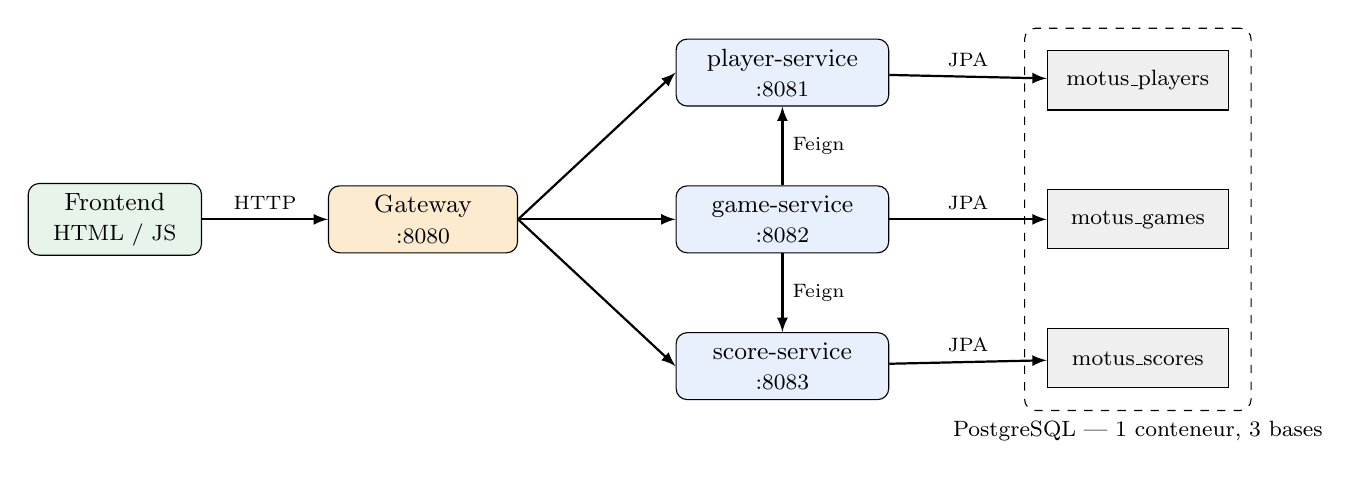
\begin{tikzpicture}[node distance=1.0cm and 1.6cm]
  \node[fe] (fe) {Frontend\\\footnotesize HTML / JS};
  \node[gw, right=of fe] (gw) {Gateway\\\footnotesize :8080};
  \node[svc, right=2cm of gw] (gs) {game-service\\\footnotesize :8082};
  \node[svc, above=of gs] (ps) {player-service\\\footnotesize :8081};
  \node[svc, below=of gs] (ss) {score-service\\\footnotesize :8083};
  \node[db, right=2cm of gs] (dbg) {motus\_games};
  \node[db, above=of dbg] (dbp) {motus\_players};
  \node[db, below=of dbg] (dbs) {motus\_scores};

  \draw[flow] (fe) -- node[above,font=\scriptsize]{HTTP} (gw);
  \draw[flow] (gw.east) -- (ps.west);
  \draw[flow] (gw.east) -- (gs.west);
  \draw[flow] (gw.east) -- (ss.west);
  \draw[flow] (ps) -- node[above,font=\scriptsize]{JPA} (dbp);
  \draw[flow] (gs) -- node[above,font=\scriptsize]{JPA} (dbg);
  \draw[flow] (ss) -- node[above,font=\scriptsize]{JPA} (dbs);
  \draw[flow] (gs) -- node[right,font=\scriptsize]{Feign} (ps);
  \draw[flow] (gs) -- node[right,font=\scriptsize]{Feign} (ss);

  \begin{pgfonlayer}{background}
    \node[draw, dashed, rounded corners, inner sep=8pt,
          fit=(dbp)(dbg)(dbs),
          label=below:{\footnotesize PostgreSQL — 1 conteneur, 3 bases}] {};
  \end{pgfonlayer}
\end{tikzpicture}
\caption{Schéma d'architecture. La gateway route \texttt{/api/players}, \texttt{/api/games}
et \texttt{/api/scores}. game-service appelle player-service (« le joueur existe-t-il ? »)
et score-service (« enregistrer le résultat »).}
\end{figure}

\textbf{Rôle des services.}
\begin{itemize}[leftmargin=1.2em, itemsep=1pt, topsep=2pt]
  \item \textbf{gateway (8080)} — Spring Cloud Gateway, point d'entrée unique, routage et CORS.
  \item \textbf{player-service (8081)} — enregistrement et gestion des joueurs (base \texttt{motus\_players}).
  \item \textbf{game-service (8082)} — logique Motus : mot mystère, validation, calcul lettre par lettre, dictionnaire (base \texttt{motus\_games}).
  \item \textbf{score-service (8083)} — historique des parties, statistiques et classement (base \texttt{motus\_scores}).
\end{itemize}

% =====================================================================
\section{Diagramme de classes « métier »}
% =====================================================================
\begin{figure}[h]
\centering
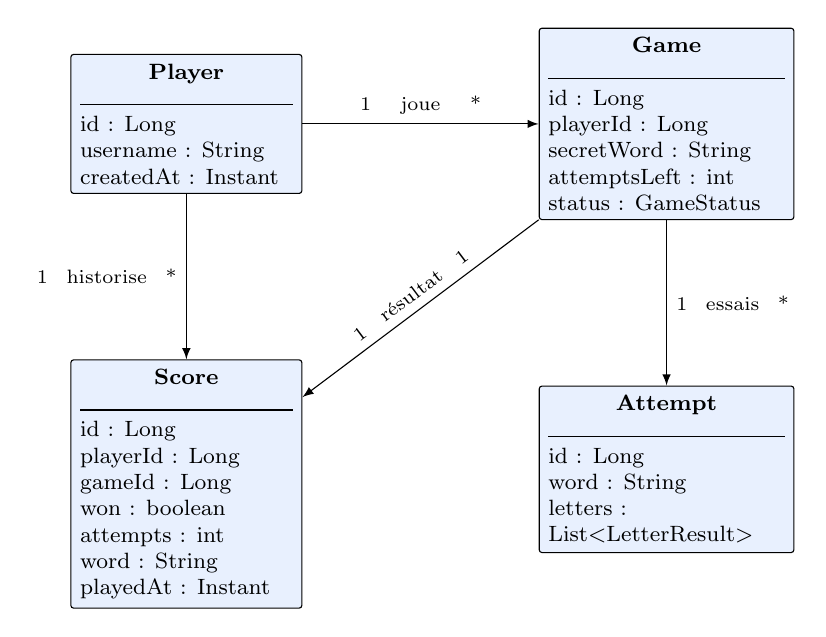
\begin{tikzpicture}[every node/.style={font=\footnotesize}]
  \tikzset{cls/.style={draw, fill=svcfill, rounded corners=1pt, align=center}}

  \node[cls] (player) {%
    \begin{minipage}{2.7cm}\centering\textbf{Player}\par\rule{\linewidth}{0.4pt}\par
    \raggedright id : Long\\ username : String\\ createdAt : Instant\end{minipage}};
  \node[cls, right=3cm of player] (game) {%
    \begin{minipage}{3cm}\centering\textbf{Game}\par\rule{\linewidth}{0.4pt}\par
    \raggedright id : Long\\ playerId : Long\\ secretWord : String\\ attemptsLeft : int\\ status : GameStatus\end{minipage}};
  \node[cls, below=2.1cm of player] (score) {%
    \begin{minipage}{2.7cm}\centering\textbf{Score}\par\rule{\linewidth}{0.4pt}\par
    \raggedright id : Long\\ playerId : Long\\ gameId : Long\\ won : boolean\\ attempts : int\\ word : String\\ playedAt : Instant\end{minipage}};
  \node[cls, below=2.1cm of game] (attempt) {%
    \begin{minipage}{3cm}\centering\textbf{Attempt}\par\rule{\linewidth}{0.4pt}\par
    \raggedright id : Long\\ word : String\\ letters : List$<$LetterResult$>$\end{minipage}};

  \draw[->,>=latex] (player) -- node[above,font=\scriptsize]{1 \quad joue \quad *} (game);
  \draw[->,>=latex] (player) -- node[left,font=\scriptsize]{1 \, historise \, *} (score);
  \draw[->,>=latex] (game) -- node[right,font=\scriptsize]{1 \, essais \, *} (attempt);
  \draw[->,>=latex] (game) -- node[above,font=\scriptsize,sloped]{1 \; résultat \; 1} (score);
\end{tikzpicture}
\caption{Entités métier et relations. \texttt{Game.secretWord} n'est jamais renvoyé au
client tant que la partie est \texttt{IN\_PROGRESS}. L'historique des essais (\texttt{Attempt})
est calculé à la volée et conservé côté client ; seul le résultat final est persisté via \texttt{Score}.}
\end{figure}

% =====================================================================
\section{Choix techniques}
% =====================================================================
\begin{table}[h]
\centering
\small
\begin{tabular}{@{}ll@{}}
\toprule
\textbf{Élément} & \textbf{Choix} \\
\midrule
Langage           & Java 21 (LTS) \\
Framework         & Spring Boot 4.0.7 \\
Spring Cloud (BOM) & 2025.1.2 (Gateway + OpenFeign) \\
Build             & Maven — un projet par service \\
Persistance       & Spring Data JPA + PostgreSQL \\
Conteneurisation  & Dockerfile multi-stage + docker-compose \\
Orchestration     & Kubernetes / MiniKube \\
Frontend          & HTML + JS vanilla, style Wordle \\
\bottomrule
\end{tabular}
\caption{Stack technique.}
\end{table}

\textbf{Justification des principaux choix :}
\begin{itemize}[leftmargin=1.2em, itemsep=1pt, topsep=2pt]
  \item \textbf{Découpage par domaine métier} (joueurs / jeu / scores) — couplage faible,
        déploiement indépendant, chaque service propriétaire de sa base.
  \item \textbf{Une seule instance PostgreSQL, trois bases logiques} — suffisant pour le
        périmètre du projet, évite la lourdeur de trois conteneurs.
  \item \textbf{OpenFeign synchrone} — simple et lisible, adapté aux flux « démarrer une
        partie » et « enregistrer un score ».
  \item \textbf{Spring Cloud Gateway} — point d'entrée unique : centralise routage et CORS.
  \item \textbf{Frontend découplé} — page statique (HTML/JS) qui n'appelle que la gateway,
        sans dépendance ni outil de build ; interface inspirée de Wordle.
  \item \textbf{Périmètre volontairement réduit} — pas d'Eureka, de Config Server ni de
        broker de messages : on privilégie la lisibilité.
\end{itemize}

% =====================================================================
\section{API REST}
% =====================================================================
Toutes les routes sont exposées via la gateway (port 8080). Réponses et erreurs au
format JSON homogène (\texttt{timestamp, status, error, message}).

\begin{table}[h]
\centering
\small
\begin{tabular}{@{}lll@{}}
\toprule
\textbf{Méthode} & \textbf{Chemin} & \textbf{Rôle} \\
\midrule
POST & \texttt{/api/players}            & Créer un joueur (201 ; 409 si pris) \\
GET  & \texttt{/api/players/\{id\}}     & Lire un joueur \\
POST & \texttt{/api/games}              & Démarrer une partie (vérifie le joueur) \\
POST & \texttt{/api/games/\{id\}/guess} & Proposer un mot (calcul des lettres) \\
GET  & \texttt{/api/games/\{id\}}       & État d'une partie (sans le mot mystère) \\
POST & \texttt{/api/scores}             & Historiser un résultat (appelé en Feign) \\
GET  & \texttt{/api/scores?playerId=}   & Historique d'un joueur \\
GET  & \texttt{/api/scores/leaderboard} & Classement \\
\bottomrule
\end{tabular}
\caption{Principaux points d'entrée de l'API.}
\end{table}

% =====================================================================
\section{Algorithme Motus}
% =====================================================================
Le cœur du jeu est le calcul lettre par lettre d'une proposition. Pour gérer
correctement les \textbf{lettres en double}, il se fait en \textbf{deux passes} :

\begin{enumerate}[leftmargin=1.4em, itemsep=1pt, topsep=2pt]
  \item \textbf{Passe 1} — pour chaque position, si la lettre proposée est identique à
        celle du mot secret au même indice, elle est \texttt{CORRECT}. Les lettres non
        encore appariées du mot secret sont comptées dans une table de fréquences.
  \item \textbf{Passe 2} — pour chaque position non \texttt{CORRECT}, si la lettre reste
        disponible dans la table, elle est \texttt{PRESENT} (et on décrémente le compteur),
        sinon \texttt{ABSENT}.
\end{enumerate}

\textit{Exemple} — mot secret \texttt{ALLER}, proposition \texttt{LELLE} :
les deux \texttt{L} de la proposition sont bornés par le nombre réel de \texttt{L}
restants après la passe~1, ce qui évite de signaler plus de lettres présentes qu'il
n'en existe réellement. Toutes les chaînes sont normalisées (majuscules, sans accents) :
le jeu est insensible à la casse et aux accents.

\textbf{Validation et dictionnaire.} Avant tout calcul, une proposition est rejetée
(message en français, sans décompter d'essai) si sa longueur diffère de celle du mot
mystère ou si le mot est inconnu. À la manière de Wordle, game-service s'appuie sur
\textbf{deux listes} : une liste restreinte de mots courants dans laquelle est tirée la
solution, et une liste beaucoup plus large de mots acceptés pour valider les
propositions. Une proposition est valable si elle figure dans l'une des deux, ce qui
permet de reconnaître bien plus de mots français tout en gardant des solutions usuelles.

% =====================================================================
\section{Frontend (page de démo)}
% =====================================================================
La page de démonstration est une application statique (HTML et JavaScript, sans
framework ni build) dont l'interface s'inspire de \textit{Wordle}. Elle ne communique
qu'avec la gateway.

Le joueur saisit ou choisit un nom, puis démarre une partie : la longueur du mot et sa
première lettre sont affichées, cette dernière apparaissant en gris clair sur la ligne
en cours pour servir d'indice. À chaque proposition, la grille se colore lettre par
lettre (vert : bien placée ; jaune : mal placée ; gris : absente) et un clavier AZERTY
reflète l'état connu de chaque lettre. En fin de partie, le mot est révélé ; une fenêtre
de statistiques présente l'historique du joueur et le classement (\texttt{/api/scores}).
Les essais ne sont pas persistés côté serveur : la page conserve les réponses reçues
pour redessiner la grille.

% --- Emplacement pour une capture du frontend ---
% \begin{figure}[h]\centering
%   \includegraphics[width=0.7\linewidth]{capture-frontend.png}
%   \caption{Page de démo : grille Motus façon Wordle et fenêtre de statistiques.}
% \end{figure}

% =====================================================================
\section{Compilation et exécution}
% =====================================================================
La procédure complète figure dans le \texttt{README.md} du dépôt. En résumé, tout se
lance via Docker Compose (PostgreSQL et ses trois bases, les services et la gateway) :

\small
\begin{verbatim}
docker compose up --build      # démarre toute la stack
# créer un joueur puis jouer :
curl -X POST localhost:8080/api/players -H 'Content-Type: application/json' \
     -d '{"username":"alice"}'
curl -X POST localhost:8080/api/games   -H 'Content-Type: application/json' \
     -d '{"playerId":1}'
curl -X POST localhost:8080/api/games/1/guess -H 'Content-Type: application/json' \
     -d '{"word":"cheval"}'
\end{verbatim}
\normalsize
La page de démo se lance ensuite avec \texttt{./serve.sh}, puis en ouvrant
\url{http://localhost:5500}. Un déploiement local sur \textbf{MiniKube} est également
prévu (un \texttt{Deployment} et un \texttt{Service} par composant, \texttt{Secret} pour
les identifiants PostgreSQL, variables d'environnement pour les URLs).

% =====================================================================
\section{Bilan}
% =====================================================================
% --- À PERSONNALISER : ces éléments sont un point de départ ---
\textbf{Réussites.} Un découpage microservices clair et homogène (un même patron repris
pour chaque service), un contrat d'API figé qui a permis aux deux binômes de travailler
en parallèle sans se bloquer, un algorithme Motus robuste aux lettres en double (validé
par des tests unitaires), et une interface web soignée inspirée de Wordle.

\textbf{Difficultés.} La gestion des doublons dans le calcul des lettres a demandé de la
rigueur (d'où l'approche en deux passes). La configuration des versions récentes
(Spring Boot 4, Spring Cloud Gateway réactif) et la communication inter-services
(gestion des pannes : enregistrement du score en « best-effort ») ont représenté
l'essentiel de l'effort de mise au point. Côté jeu, le dictionnaire initial, trop
restreint, refusait des mots français corrects : nous l'avons remplacé par deux listes
(mots courants pour la solution, large liste pour la validation).

\textbf{Ce que nous avons appris.} L'architecture microservices et ses compromis,
Spring Cloud Gateway, OpenFeign, la conteneurisation multi-stage avec Docker, la
persistance JPA multi-bases et le déploiement sur MiniKube.

\textbf{Ce que nous avons le plus / le moins aimé.} Nous avons apprécié la modularité et
l'autonomie de chaque service ; la contrepartie a été la lourdeur de configuration et de
débogage propre aux échanges inter-services.

\end{document}
